\documentclass[notes,10.2pt, aspectratio=169]{beamer}

\usepackage{pgfpages}
% These slides also contain speaker notes. You can print just the slides,
% just the notes, or both, depending on the setting below. Comment out the want
% you want.
\setbeameroption{hide notes} % Only slide
%\setbeameroption{show only notes} % Only notes
% \setbeameroption{show notes on second screen=right} % Both

\usepackage{import}
\usepackage{helvet}
% \usepackage[default]{lato}
\usepackage{array}
% \usepackage{natbib}
% \bibliographystyle{plain}
\usepackage{apalike}
\bibliographystyle{apalike}
% \usepackage[natbib, maxcitenames=3, mincitenames=11, style=apa]{biblatex}

\usepackage{tikz}
\newcommand*\circled[4]{\tikz[baseline=(char.base)]{
    \node[shape=circle, fill=#2, draw=#3, text=#4, inner sep=2pt] (char) {#1};}}
\usepackage{verbatim}
\setbeamertemplate{note page}{\pagecolor{yellow!5}\insertnote}
\usetikzlibrary{positioning}
\usetikzlibrary{snakes}
\usetikzlibrary{calc}
\usetikzlibrary{arrows}
\usetikzlibrary{decorations.markings}
\usetikzlibrary{shapes.misc}
\usetikzlibrary{matrix,shapes,arrows,fit,tikzmark}
\usepackage{amsmath}
\usepackage{mathpazo}
\usepackage{hyperref}
\usepackage{lipsum}
\usepackage{multimedia}
\usepackage{graphicx}
\usepackage{multirow}
\usepackage{graphicx}
\usepackage{dcolumn}
\usepackage{bbm}
\usepackage{cancel}
\newcolumntype{d}[0]{D{.}{.}{5}}
\usepackage{subcaption}
\usepackage{changepage}
\usepackage{appendixnumberbeamer}
\newcommand{\beginbackup}{
   \newcounter{framenumbervorappendix}
   \setcounter{framenumbervorappendix}{\value{framenumber}}
   \setbeamertemplate{footline}
   {
     \leavevmode%
     \hline
     box{%
       \begin{beamercolorbox}[wd=\paperwidth,ht=2.25ex,dp=1ex,right]{footlinecolor}%
%         \insertframenumber  \hspace*{2ex} 
       \end{beamercolorbox}}%
     \vskip0pt%
   }
 }
\newcommand{\backupend}{
   \addtocounter{framenumbervorappendix}{-\value{framenumber}}
   \addtocounter{framenumber}{\value{framenumbervorappendix}} 
}


\usepackage{graphicx}
\usepackage[space]{grffile}
\usepackage{booktabs}

% These are my colors -- there are many like them, but these ones are mine.
% \definecolor{blue}{RGB}{20,160,210}
\definecolor{blue}{RGB}{80,150,170}
\definecolor{red}{RGB}{213,94,0}
\definecolor{yellow}{RGB}{240,228,66}
\definecolor{green}{RGB}{0,158,115}

% % Enviroments
% \newtheorem{defin}{Definition.}
% \newtheorem{teo}{Theorem. }
% \newtheorem{lema}{Lemma. }
% \newtheorem{coro}{C
% \begin{frame}{Modeling Choice}orolary. }
% \newtheorem{prop}{Proposition. }
% \theoremstyle{definition}
% \newtheorem{examp}{Example. }
% % \numberwithin{problem}{subsection} 

\hypersetup{
  colorlinks=false,
  linkbordercolor = {white},
  linkcolor = {blue}
}


%% I use a beige off white for my background
\definecolor{MyBackground}{RGB}{255,253,218}

%% Uncomment this if you want to change the background color to something else
%\setbeamercolor{background canvas}{bg=MyBackground}

%% Change the bg color to adjust your transition slide background color!
\newenvironment{transitionframe}{
  \setbeamercolor{background canvas}{bg=white}
  \begin{frame}}{
    \end{frame}
}

\setbeamercolor{frametitle}{fg=blue}
\setbeamercolor{title}{fg=black}
\setbeamertemplate{footline}[frame number]
\setbeamertemplate{navigation symbols}{} 
%\setbeamertemplate{itemize items}{-}
\setbeamercolor{itemize item}{fg=blue}
\setbeamercolor{itemize subitem}{fg=blue}
\setbeamercolor{enumerate item}{fg=blue}
\setbeamercolor{enumerate subitem}{fg=blue}
\setbeamercolor{button}{bg=MyBackground,fg=blue,}
\setbeamercolor{theotem}{fg=blue} 

% If you like road maps, rather than having clutter at the top, have a roadmap show up at the end of each section 
% (and after your introduction)
% Uncomment this is if you want the roadmap!
%\AtBeginSection[]
%{
%   \begin{frame}
%       \frametitle{Roadmap of Talk}
%       \tableofcontents[currentsection]
%   \end{frame}
%}


\setbeamercolor{section in toc}{fg=blue}
\setbeamercolor{subsection in toc}{fg=red}
\setbeamersize{text margin left=1em,text margin right=1em} 

\newenvironment{wideitemize}{\itemize\addtolength{\itemsep}{10pt}}{\enditemize}

\usepackage{environ}
\NewEnviron{videoframe}[1]{
  \begin{frame}
    \vspace{-8pt}
    \begin{columns}[onlytextwidth, T] % align columns
      \begin{column}{.58\textwidth}
        \begin{minipage}[t][\textheight][t]
          {\dimexpr\textwidth}
          \vspace{8pt}
          \hspace{4pt} {\Large \sc \textcolor{blue}{#1}}
          \vspace{8pt}
          
          \BODY
        \end{minipage}
      \end{column}%
      \hfill%
      \begin{column}{.42\textwidth}
        \colorbox{green!20}{\begin{minipage}[t][1.2\textheight][t]
            {\dimexpr\textwidth}
            Face goes here
          \end{minipage}}
      \end{column}%
    \end{columns}
  \end{frame}
}

\title[]{\textcolor{blue}{Many Markets Make Good Neighbors: Multimarket Contact and Deposit Banking  \\ Hatfield and Wallen (2023)}}

\author{ Presenter: Giselle Labrador Badia}
%\centering
\date{\today}


\begin{document}
%%% TIKZ STUFF
\tikzset{   
        every picture/.style={remember picture,baseline},
        every node/.style={anchor=base,align=center,outer sep=1.5pt},
        every path/.style={thick},
        }
\newcommand\marktopleft[1]{%
    \tikz[overlay,remember picture] 
        \node (marker-#1-a) at (-.3em,.3em) {};%
}
\newcommand\markbottomright[2]{%
    \tikz[overlay,remember picture] 
        \node (marker-#1-b) at (0em,0em) {};%
}
\tikzstyle{every picture}+=[remember picture] 
\tikzstyle{mybox} =[draw=black, very thick, rectangle, inner sep=10pt, inner ysep=20pt]
\tikzstyle{fancytitle} =[draw=black,fill=red, text=white]
%%%% END TIKZ STUFF

% % Title Slide
\begin{frame}
  \maketitle
\end{frame}
% % % Outline Slide
% \begin{frame}
%   \frametitle{Roadmap of Talk}
%   \tableofcontents
% \end{frame}

% INTRO
% \section{Motivation}


% \begin{frame}{Motivation}

%   \begin{figure}[t*]
%   %   \begin{subfigure}[t]{0.45\textwidth}
%   %     \label{fig:fig1}
%   %   \includegraphics[width=1\textwidth]{/Users/gisellelab/Work/deposit_pricing/document/imgs/boa_2010.pdf}
%   %   \caption{Bank of America}
%   %   \end{subfigure}\hfill
  
%   %   \begin{subfigure}[t]{0.45\textwidth}
%   %     \label{fig:fig2}
%     \includegraphics[width=.4\textwidth]{/Users/gisellelab/Work/deposit_pricing/document/imgs/wf_2010.pdf}
%     \caption{Wells Fargo}
%   %   \end{subfigure}
%   \end{figure}
  
%   \end{frame}
  
   

\begin{frame}[noframenumbering]
  \textcolor{blue}{\huge{\centerline{Introduction}}}

\end{frame}

    
\begin{frame}{Motivation and Goal}
\begin{wideitemize}
    \item Industry concentration has increased at the national level, but decreasing at the local level (Ksieh and Rossi-Hansberg (2021), Rossie-Hansberg et al. (2021)). 
    \item If local is the relevant measure, why have markups and profitability increased? (De Loecker et al. (2020), Barkai (2020))
    \item Firms behave less competitively even though they face more competition.
    \pause
    \item \textbf{This paper proposes that multimarket contact can explain this puzzle.}
    \vspace{0.2cm}
    \begin{wideitemize}
      \item Build model that shows an increase in multimarket contact leads firms to behave less competitively. 
      \item Empirically show this relationship in the deposit market. 
    \end{wideitemize}

\end{wideitemize}
    
\end{frame}

% \begin{frame}{Motivation}

%     \begin{wideitemize}
%     \item The impact of increasing the reserve supply on bank lending is ambiguous: 
%     \vspace{0.15cm}
%     \begin{wideitemize}
%         \item[$\uparrow$] \textit{lending:} \\Reduce costs of selling illiquid assets in a bank run (Diamond and Dybvig, 1983), \\
%          help complies with liquidity regulations.  
%         \item[$\downarrow$] \textit{lending:} \\ cost of meeting capital requirements when equity is scarce (Kashyap and Stein 1993),  \\
%         amplify liquidity strains during stress episodes (Acharya and Rajan, 2021),\\
%         bank leverage regulation can make it costly to expand asset holding (Du, Tepper, and Verdelhan, 2018)    
%     \end{wideitemize}
    
%     \end{wideitemize}
    
%     \end{frame}
    

\begin{frame}{Motivation and Goal}
    \vspace{0.5cm}
      \begin{itemize}
        \item  The decrease in passthrough is evidence of an increase in market power in the deposit market.

      \end{itemize}

      % TODO: add figure of passthrough figure 1
      
                \begin{figure}[t*]
          \centering
          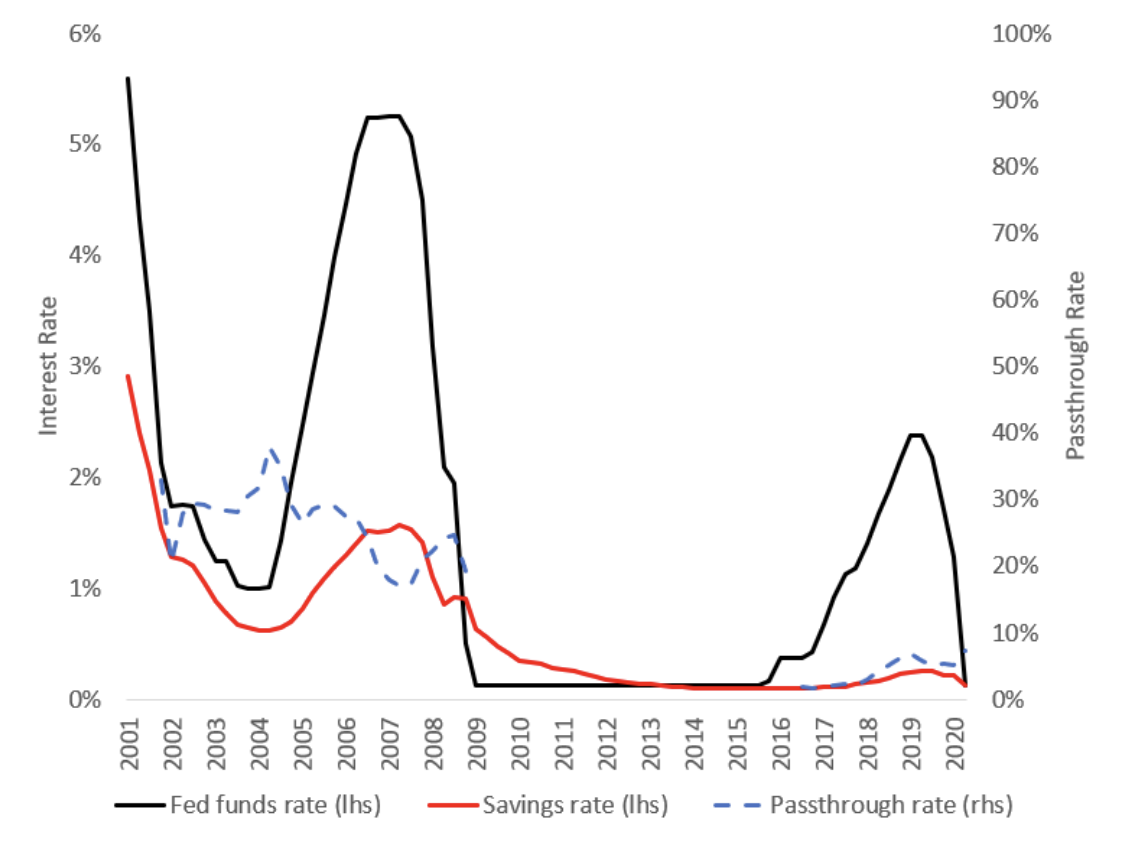
\includegraphics[width=.58\textwidth]{./imgs/figure1}
        % \caption{Supply of Central Banks Reserves and Bank Asset Illiquidity}
        \end{figure}


      \end{frame}
    


\begin{frame}{Preview of Results}

    \vspace{0.5cm}
      \begin{wideitemize}

      \item \textbf{Model:} Multimarket contact leads to less competitive behavior.
      \vspace{0.2cm}
      \begin{itemize}
        \item Mergers lead to worse consumer outcomes even if they do not increase local concentration.
        \item Markups are positively correlated with higher local concentration and multimarket contact.
      \end{itemize}
      \pause
      \item \textbf{Empirical Analysis:} 
      \vspace{0.2cm}
      \begin{itemize}
        \item In the deposit market, multimarket contact enables banks to behave as if the local market was twice as concentrated. 
        \item Estimate that markups have increased by 27\% for retail industries while the propensity for retail networks to overlap has more than tripled. 
      \end{itemize}
    \end{wideitemize}
      \end{frame}
    



\section{Related Literature}
\begin{frame}[label = lit]{Related Literature}

  \begin{wideitemize}
      \item \textbf{Multimarket contact and collusive behavior.}
      \vspace{0.2cm}
      \begin{wideitemize}
    
        \item Bernheim and Whinston (1990) formalize the idea that multimarket contact can facilitate collusion.
        \item Empirical evidence: Busse (2000), celular phones;
        Ciliberto and Williams (2014), airlines;
        Jans and Rosenbaum (1990), cement;
        Fernandez and Marin (1998), hotels;
        Schmitt (2018), hospitals.
        
      \end{wideitemize}


          \item \textbf{Concentration and anticompetitive behavior in the banking industry.}
          \vspace{0.2cm}
          \begin{wideitemize}
            \item  Dreschsler et al (2017), Granja and Paixão (2020), Corbae and D'Erasmo (2020, 2021).
            \item Collusive behavior in asset markets: Duffie and Stein (2015), LIBOR;  Cai and Jahanshahloo (2019) foreign exchange market. 
          \end{wideitemize}
      

  \end{wideitemize}
  
\end{frame}

% \section{Background and Data}


% \begin{frame}[label = backg]{Background}



% \begin{itemize}
%     \item 
    
%     \item  \hyperlink{backg_col_diagram_appendix}{\beamergotobutton{C}}
%     \begin{itemize}
%         \item 
%     \end{itemize}
    
%     \item 
%     \end{itemize}

% \end{frame}






\begin{frame}[noframenumbering]
    \textcolor{blue}{\huge{\centerline{Theory}}}

\end{frame}


% \begin{frame}
%     \textcolor{blue}{\huge{\centerline{Model of Bank Balance Sheets}}}

% \end{frame}


\begin{frame}{Model: Market Structure}
    \vspace{0.2cm}
Bertrand competition model with $M$ markets, $F$ firms.
\vspace{0.2cm}
\begin{wideitemize}
    \item Market structure $k \in \{ 0, 1\}^{F,M}$, where $k_{f m}=1$ if firm $f$ operates in market $m$. 
    \item $f$ is \textit{national} if $k_{f m}=1$ for more than one $m$.
    \item $f$ is \textit{local} if $k_{f m}=1$ for only one $m$.
    \item A \textit{merger} where $f$ adquires $\hat{f}$ is a change in $k$ where $k^f_m=1$ for all $m$ of the acquired firm, and $k^{\hat{f}}_m=0$ for all $m$.
    \item A \textit{market extension merger} where for all $m$ either $k^f_m=0$ for all $m$ of the acquired firm, and $k^{\hat{f}}_m=0$.

\end{wideitemize}

    \end{frame}
    
\begin{frame}{Model: The Stage Game}

  \begin{wideitemize}

\item Each firm $f$ chooses a price $p_^f_m \in [0, \infty]$ and an aggresiveness $a^f_m \in [0, \infty]$ in each market $m$..
\item The quantity demanded of firm $f$  by consumers in market $m$  is:

$$Q_m^f\left(p_m, a_m\right) \equiv \psi_m D\left(\min _{\bar{f} \in F}\left\{p_m^{\bar{f}}\right\}\right) \times \mathbb{1}_{\left\{f \in \mathbf{A}_m\left(r_m\right)\right\}} \frac{a_m^b}{\sum_{\bar{f} \in \mathbf{A}_m\left(p_m\right)} a_m^{\bar{f}}}$$

where $\psi_m$ is the market size, $D$ is a strictly decreasing and concave demand, $\mathbf{A}_m\left(p_m\right)$ is the set of firms with the lower price in $m$ and $r_m$ is the set of firms that operate in $m$.

\pause 

\item Profits of firm $f$ in market $m$ are:

$$\Pi^f\left(p, a\right)= \sum_{m \in M}  Q_m^f\left(p_m, a_m\right) (p_m^f -c)$$

where $c$ is the marginal cost of production.
\end{wideitemize}
  

\end{frame}


\begin{frame}{Model: The Repeated Game}

  \begin{wideitemize}

  \item $p^{\circ}$ is the stage game monopoly price.
  \item \textbf{In the stage game}, if more than one firm operates in each market, then each firm obtains profits zero in every pure Nash equilibrium.
  \item \textbf{In an economy with one market}, If $|\mathbf{F}(m)| \leq \frac{1}{1-\delta}$ then any price $p \in\left[c, p^{\circ}\right]$ is sustainable; otherwise only $p=c$ is sustainable.
  
  \item \textbf{In the multimarket economy},  prices $p$ and quantities $q$ are substained if: 

$$
\frac{1}{1-\delta} \sum_{m \in M}\left(p_m-c\right) q_m^f \geq \sum_{m \in M}\left(p_m-c\right) \psi_m D\left(p_m\right) \text{ for each firm $f$}, 
$$

$$
\text{and } \sum_{f \in F} q_m^f=\psi_m D\left(p_m\right) \text{for each market $m$}.
$$

\end{wideitemize}
  

\end{frame}


\begin{frame}{Merger ramifications, multimarket contact and competition}



  \begin{wideitemize}

  \item \textbf{Theorem 1:} Let $\hat{\kappa}$ be a merger under $\kappa$ and suppose that $\hat{\kappa}$ is sufficient for competition: Then any prices sustainable under $\kappa$ are also sustainable under $\hat{\kappa}$.
  \begin{itemize}
  \item \textcolor{blue}{The price is never lower after a merger even if the merger is a market extension merger.} 
  \end{itemize}
  
  \pause 

  \item \textbf{Theorem 2:}  Suppose that for two markets $m$ and $n$ of equal size, less local firms in market $m$, and same national firms in both markets, then 
  \textit{In any highest-profit equilibrium for national firms, $p_m \geq p_n$.}. 
  \begin{itemize}
    \item \textcolor{blue}{ If the market is less competitive, then it has a higher price.} 
    \end{itemize}
    
  \pause 

  \item \textbf{Theorem 3:}  Suppose that for two markets $m$ and $n$ of equal size, less firms in market $m$, and all national firms in $n$ also in $m$, then
  \textit{In any highest-profit equilibrium for national firms, $p_m \geq p_n$.}.
  \begin{itemize}
    \item \textcolor{blue}{ If the market has more multimarket contact, then it has a higher price.} 
    \end{itemize}


\end{wideitemize}
  

\end{frame}


\begin{frame}{  Deposit Banking Model}
  \vspace{0.2cm}
% Bertrand competition model with $M$ markets, $F$ firms.
% \vspace{0.2cm}
\begin{wideitemize}
  \item Capacity $k \in \{ 0, \psi_m\}^{F,M}$.

  \item Merger results in a new capacity $k^{\hat{f}}_m = k^f_m + k^{\hat{f}}_m$.
  \item Consumer's demand depend on FED rate $f$ and preference for liquidity $\lambda$:
  $$D(r, f) \equiv(1+\lambda) \frac{r}{f+\lambda r}$$
  \item Quantity of consumers of bank $b$ in market $m$ is:
  $$Q_m^b\left(r_m, a_m\right) \equiv \psi_m \mathbb{1}_{\left\{b \in \mathbf{A}_m\left(r_m\right)\right\}} \frac{a_m^b}{\sum_{\bar{b} \in \mathbf{A}_m\left(r_m\right)}^b a_m^{\bar{b}}}$$.
  \item Profits of bank $b$ in market $m$ are:
  $$\Pi_m^b\left(r_m, a_m, f\right) \equiv {Q_m^b\left(r_m, a_m\right)} D\left(r_m^b, f\right) \left(f-r_m^b\right) -c \underbrace{\max \left\{0, Q_m^b\left(r_m, a_m\right)-\kappa_m^b\right\}}_{\text{Consumers over capacity}}$$.

\end{wideitemize}

  \end{frame}
  
\begin{frame}{ Deposit Banking Model: Merger ramifications, multimarket contact and competition}
  \begin{wideitemize}

    \item \textbf{Theorem 1:} 
    \begin{itemize}
    \item \textcolor{blue}{The profits are never lower after a merger even if the merger is a market extension merger.} 
    \end{itemize}
    
    \pause 
  
    \item \textbf{Theorem 2:}  In markets that only differ in local concentration, 
    \begin{itemize}
      \item \textcolor{blue}{ if the market is less competitive (lower capacity), then it has a higher spread and higher capture rate.} 
      \end{itemize}
      
    \pause 
  
    \item \textbf{Theorem 3:} In markets that only differ in multimarket contact, 
    \begin{itemize}
      \item \textcolor{blue}{ If the market has more multimarket contact, then it has a higher spread and higher capture rate.} 
      \end{itemize}
  
  
  \end{wideitemize}
\end{frame}

    
\begin{frame}{ Deposit Banking}
  \begin{wideitemize}

     \item $r^*_n$ in dark green, $r^*_m$ in dash red, consumer demand in light green. 
     % Figure 8
          \begin{figure}[t*]
          \centering
          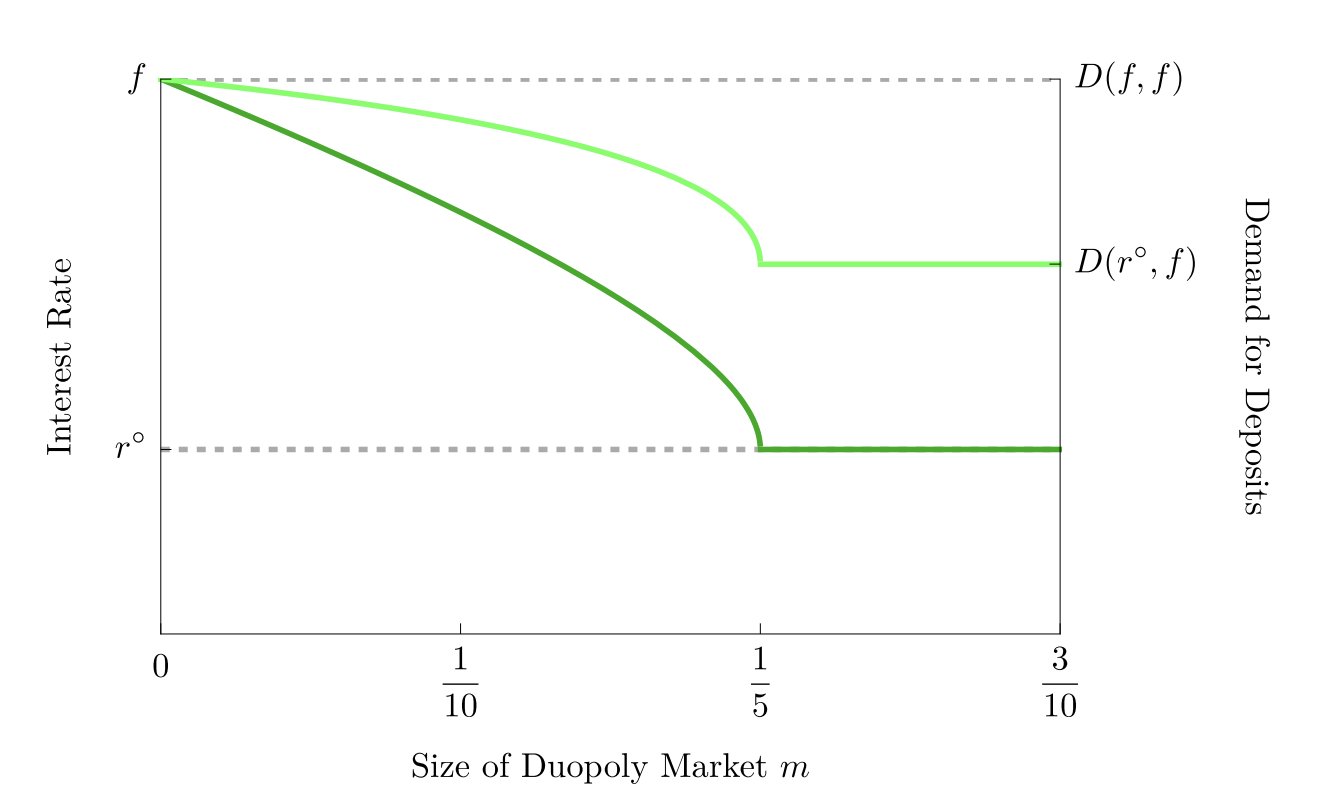
\includegraphics[width=.7\textwidth]{./imgs/figure8.png}
        % \caption{Supply of Central Banks Reserves and Bank Asset Illiquidity}
        \end{figure}

  
  \end{wideitemize}
\end{frame}

    
\begin{frame}{ Deposit Banking}
  \begin{wideitemize}

    \item $r^*_n$ in dark green, $r^*_m$ in dash red, consumer demand in light green. 
    %  Figure 9
    \begin{figure}[t*]
      \centering
      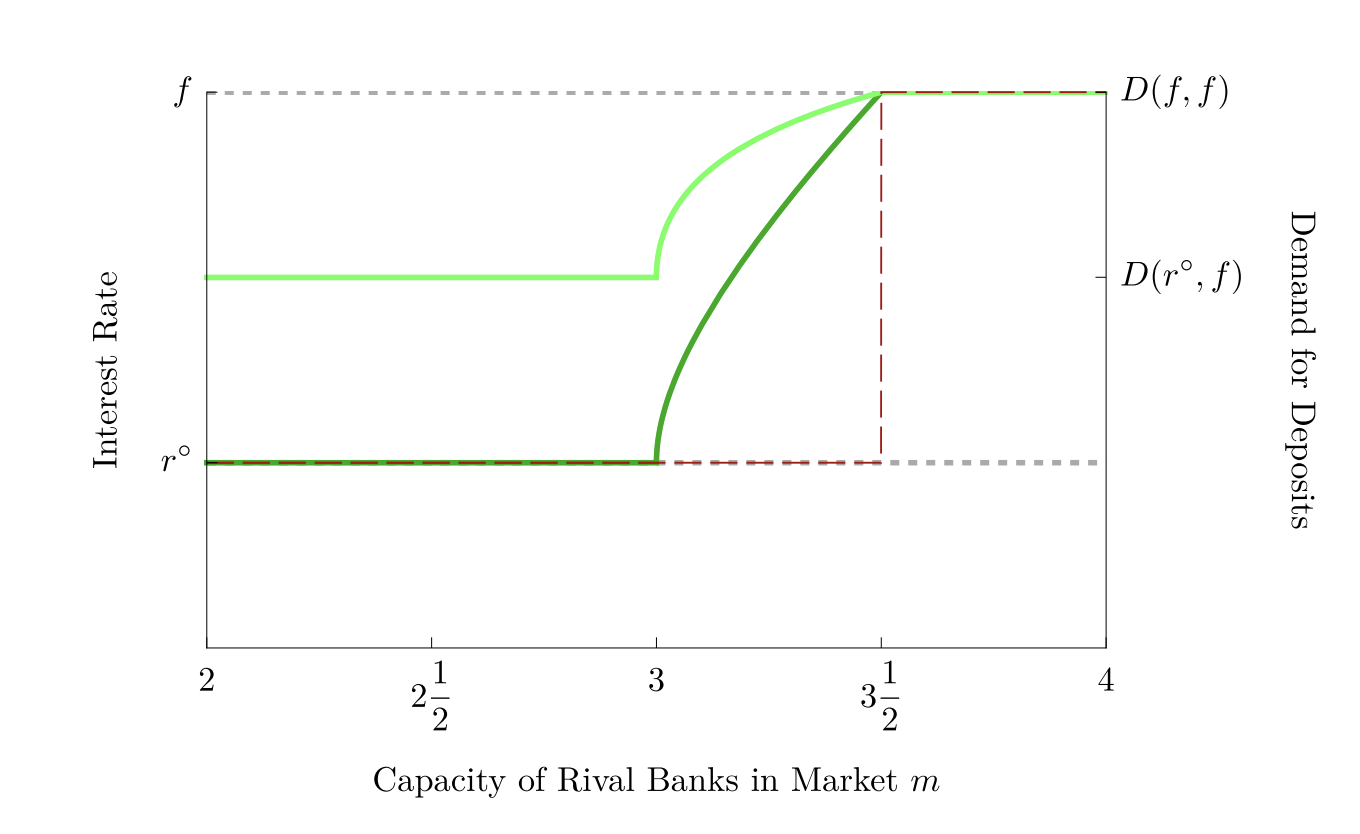
\includegraphics[width=.7\textwidth]{./imgs/figure9.png}
    % \caption{Supply of Central Banks Reserves and Bank Asset Illiquidity}
    \end{figure}

  
  \end{wideitemize}
\end{frame}


\begin{frame}[noframenumbering]
    \textcolor{blue}{\huge{\centerline{Empirical Analysis}}}
\end{frame}

\begin{frame}{Data and Definitions}
    \vspace{0.2cm}

    \begin{wideitemize}

    \item SOD data: 2019 counties, 146 banks.
    \item RateWatch: deposit interest rate, use only rate-setting branches. 
    \item Multimarket contact between banks $i$ and $j$ in market $m$:
    $$\mathrm{MMC}_{i, j} \equiv \sum_c\left(\theta_c^i \cdot \theta_c^j\right)^{\frac{1}{2}}$$
    where $\theta_c^i \equiv \frac{q_c^i}{\sum_{\bar{c}} q_{\bar{c}}^i}$ be the sales portfolio share of firm $i$ in market $c$.

    \item Multimarket contact in county $c$:
    $$\mathrm{MMC}_c \equiv \frac{\sum_i \sum_{j \neq i} \mathrm{MMC}_{i, j} q_c^i q_c^j}{\sum_i \sum_{j \neq i} q_c^i q_c^j}$$.

  \end{wideitemize}
\end{frame}

\begin{frame}{Deposit spread}
    \vspace{0.1cm}
    \begin{wideitemize}
    \item Bank market power is measured by deposit spread beta: 
    $$\Delta y_{b, t}=\alpha_b+\beta \Delta \mathrm{FF}_t+\epsilon_{b, t}$$
    where $\Delta y_{b, t}$ is the change in the deposit spread and $\Delta \mathrm{FF}_t$ is the change in the FED rate.


% TODO:  Table 1
\begin{figure}[t*]
  \centering
  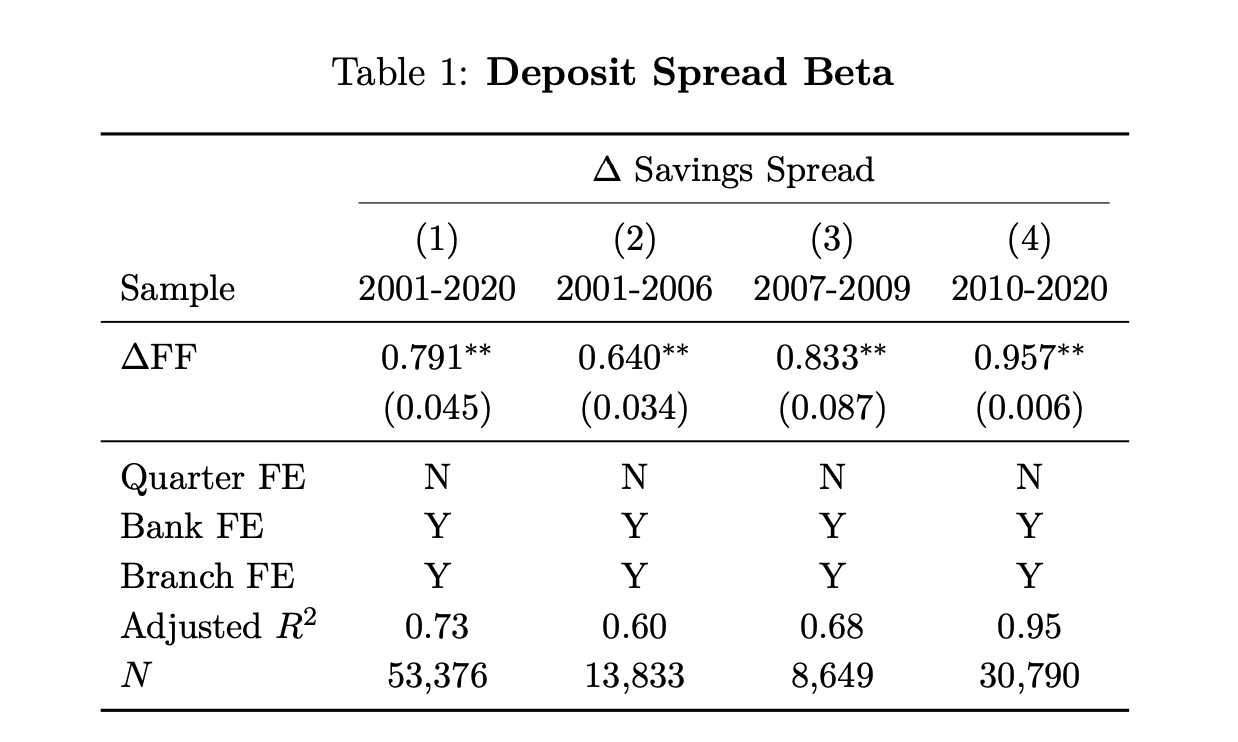
\includegraphics[width=.65\textwidth]{./imgs/table1.png}
% \caption{Supply of Central Banks Reserves and Bank Asset Illiquidity}
\end{figure}



\end{wideitemize}

\end{frame}


\begin{frame}{Deposit spread: Across Bank-Branches Estimates}
  \vspace{0.1cm}
  \begin{wideitemize}
  \item For each branch $b$ in market $m$, estimate:
  $$\Delta y_{b, t}=\alpha_b+\beta_b \Delta \mathrm{FF}_t+\epsilon_{b, t}$$
  where $\Delta y_{b, t}$ is the change in the deposit spread and $\Delta \mathrm{FF}_t$ is the change in the FED rate.

  

% TODO:  Figure 6
\begin{figure}[t*]
  \centering
  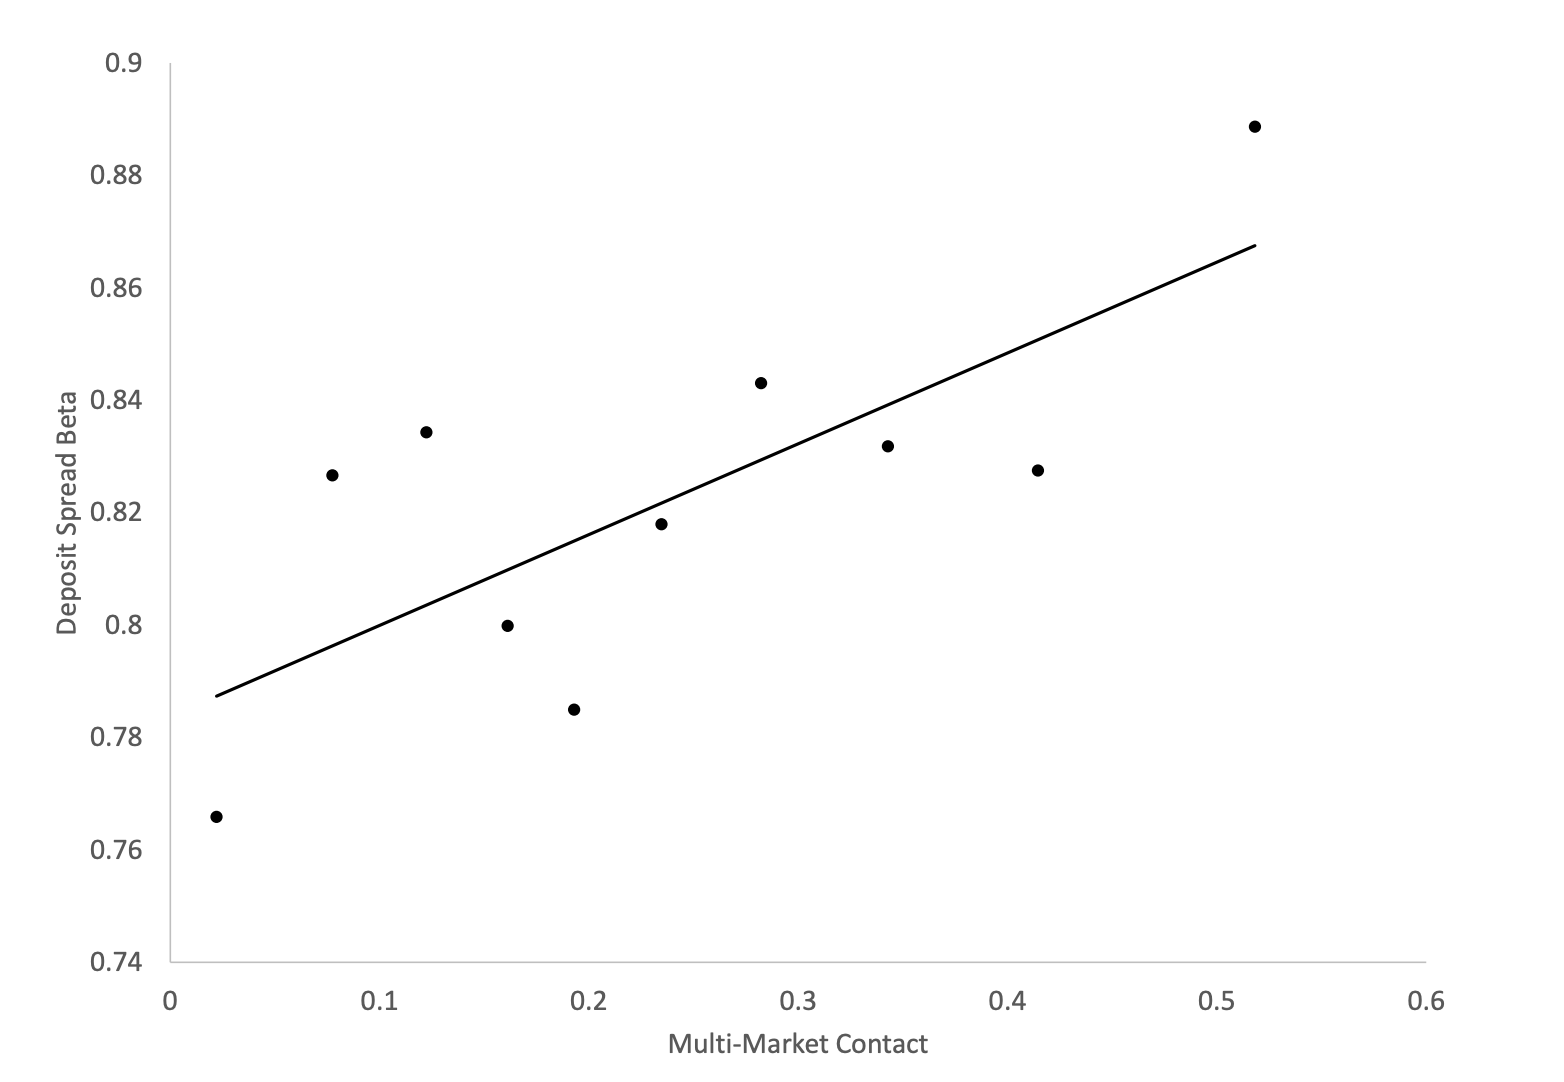
\includegraphics[width=.5\textwidth]{./imgs/figure6.png}
% \caption{Supply of Central Banks Reserves and Bank Asset Illiquidity}
\end{figure}



\end{wideitemize}

\end{frame}

\begin{frame}{Within-bank and Across-County Estimates}
  \vspace{0.1cm}
  \begin{wideitemize}
  \item $\Delta y_{b, t}=\alpha_t+\alpha_b+\zeta_{s(b), t}+\chi_{i(b), t}+\gamma \Delta \mathrm{FF}_t \times \mathrm{MMC}_{c(b), t}+\epsilon_{b, t}$
  

% TODO:  Table 2
\begin{figure}[t*]
  \centering
  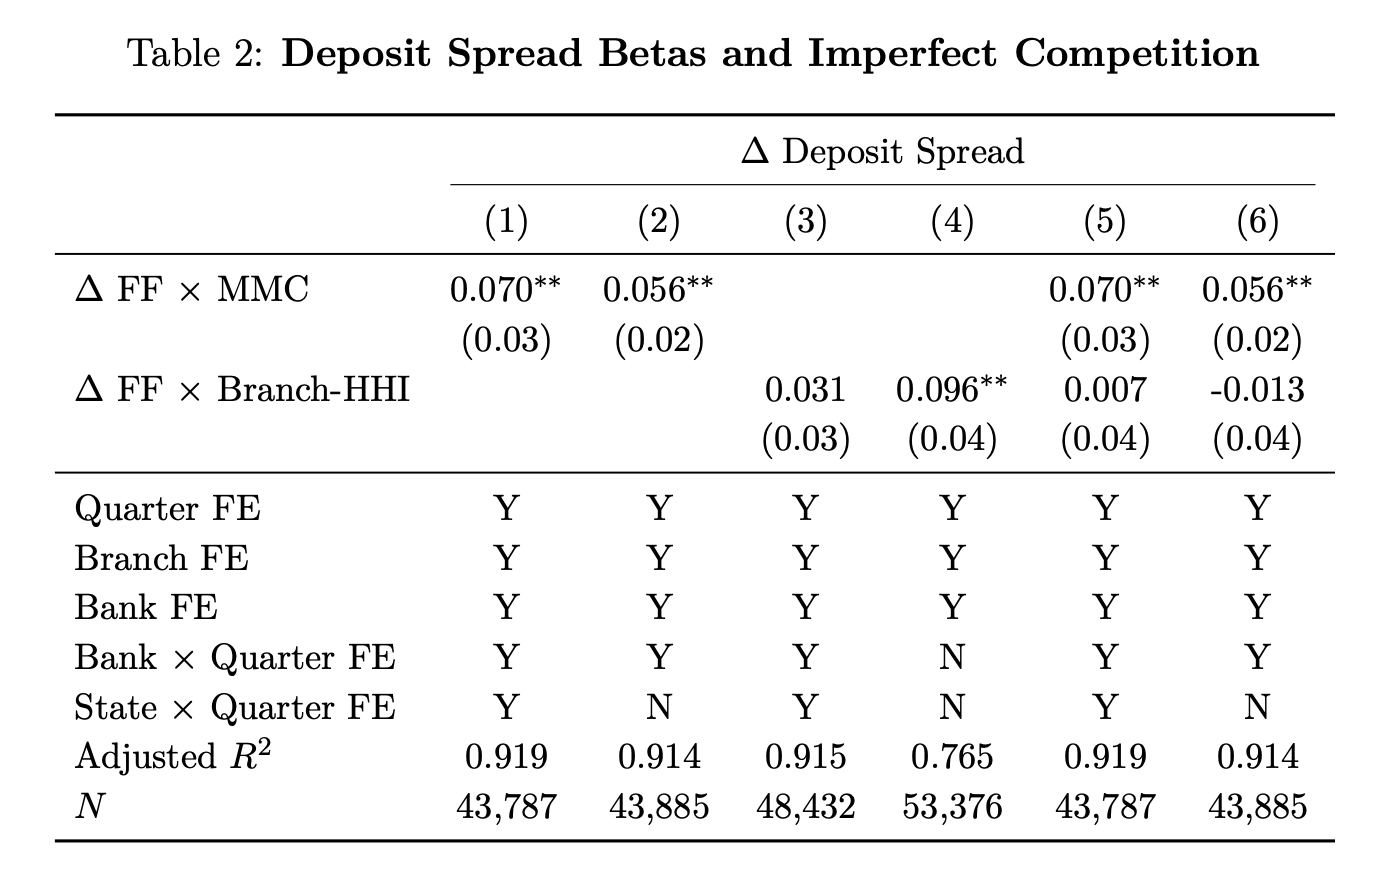
\includegraphics[width=.68\textwidth]{./imgs/table2.png}
% \caption{Supply of Central Banks Reserves and Bank Asset Illiquidity}
\end{figure}

\end{wideitemize}

\end{frame}


\begin{frame}{Deposit Market Contact and Merger Activity}
  \vspace{0.1cm}
  \begin{wideitemize}
  \item The Network $\mathrm{MMC}_{i, j}$ of acquiring bank $i$ and target bank $j$ is
  $$
  \text { Network } \mathrm{MMC}_{i, j}=\frac{\sum_{n \neq i} \mathrm{MMC}_{i, n} q_{c(n)}^j}{\sum_n q_{c(n)}^j}
  $$
  where $n$ are other national banks,  $\mathrm{MMC}_{i, n}$ is the multimarket contact of $i$  and $n$, and $q_{c(n)}^j$ is the quantity of target bank $j$ 's deposits that overlap with $n$. 

  \item We estimate the association between mergers and multimarket contact:
  $$
  \operatorname{Merger}_{i, j, t}=\alpha_{i, t}+\beta \text { Network } \mathrm{MMC}_{i, j}+\xi X_{i, j, t}+\epsilon_{i, j, t},
  $$
  where $\alpha_{i, t}$ is an acquirer bank-by-time fixed effect and $X_{i, j, t}$ are control variables.


\end{wideitemize}
\end{frame}

\begin{frame}{Deposit Market Contact and Merger Activity}
  \vspace{0.1cm}

% TODO:  Table 3

\begin{figure}[t*]
  \centering
  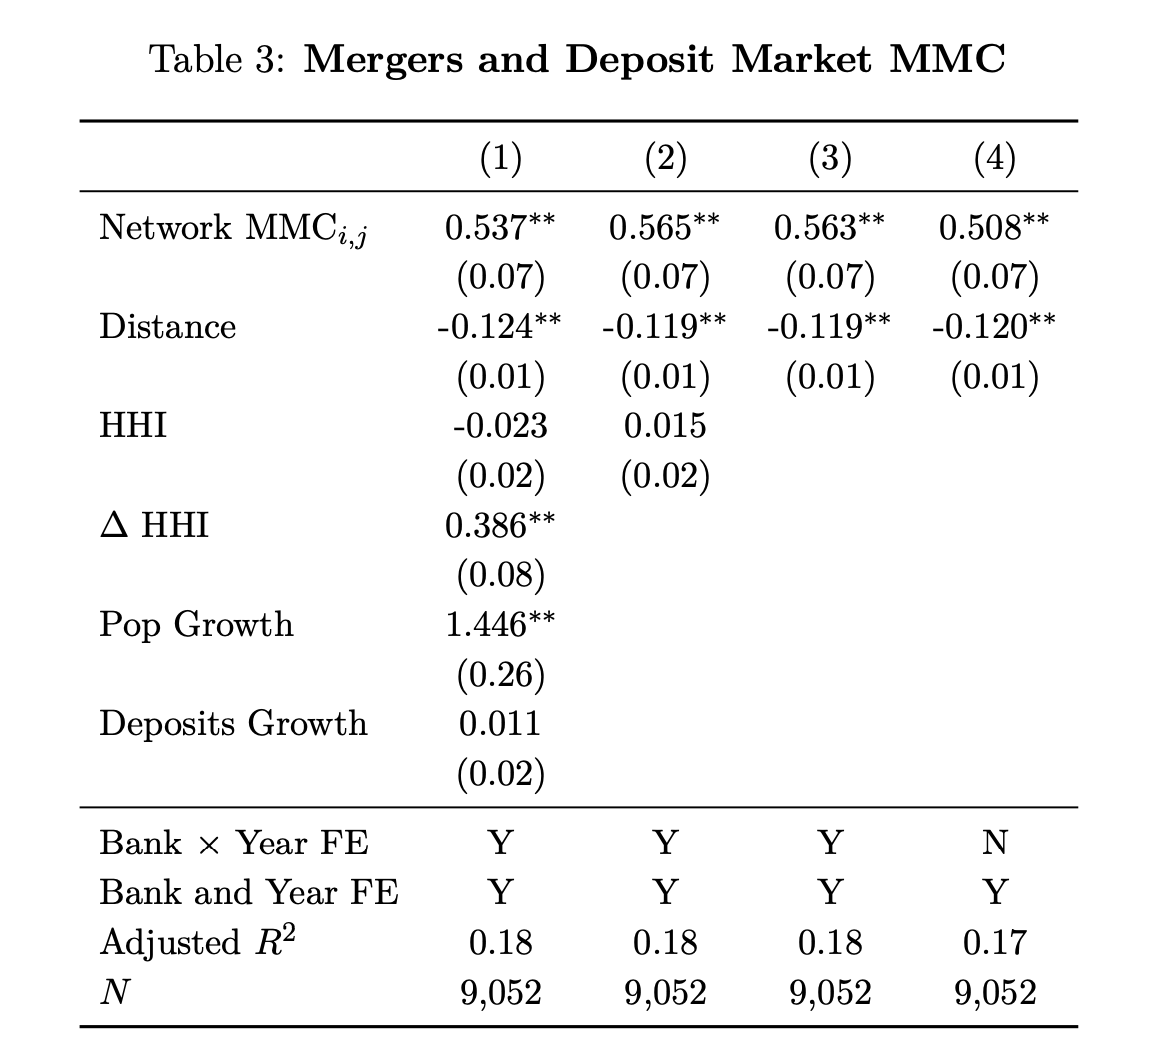
\includegraphics[width=.55\textwidth]{./imgs/table3.png}
% \caption{Supply of Central Banks Reserves and Bank Asset Illiquidity}
\end{figure}


\end{frame}

\begin{frame}{Deposit Market Branch Warfare}

  \begin{wideitemize}
  \item $
  y_{b, t}=\alpha_t+\beta_t T_{c(b)}+\epsilon_{b, t},
  $\\
  where $y_{b, t}$ is the deposit spread for branch $b$, and $T_{c(b)}$ is 1 if Wells Fargo or JP Morgan Chase has a branch in the county of branch $b$.
\end{wideitemize}

% TODO:  Figure 7

\begin{figure}[t*]
  \centering
  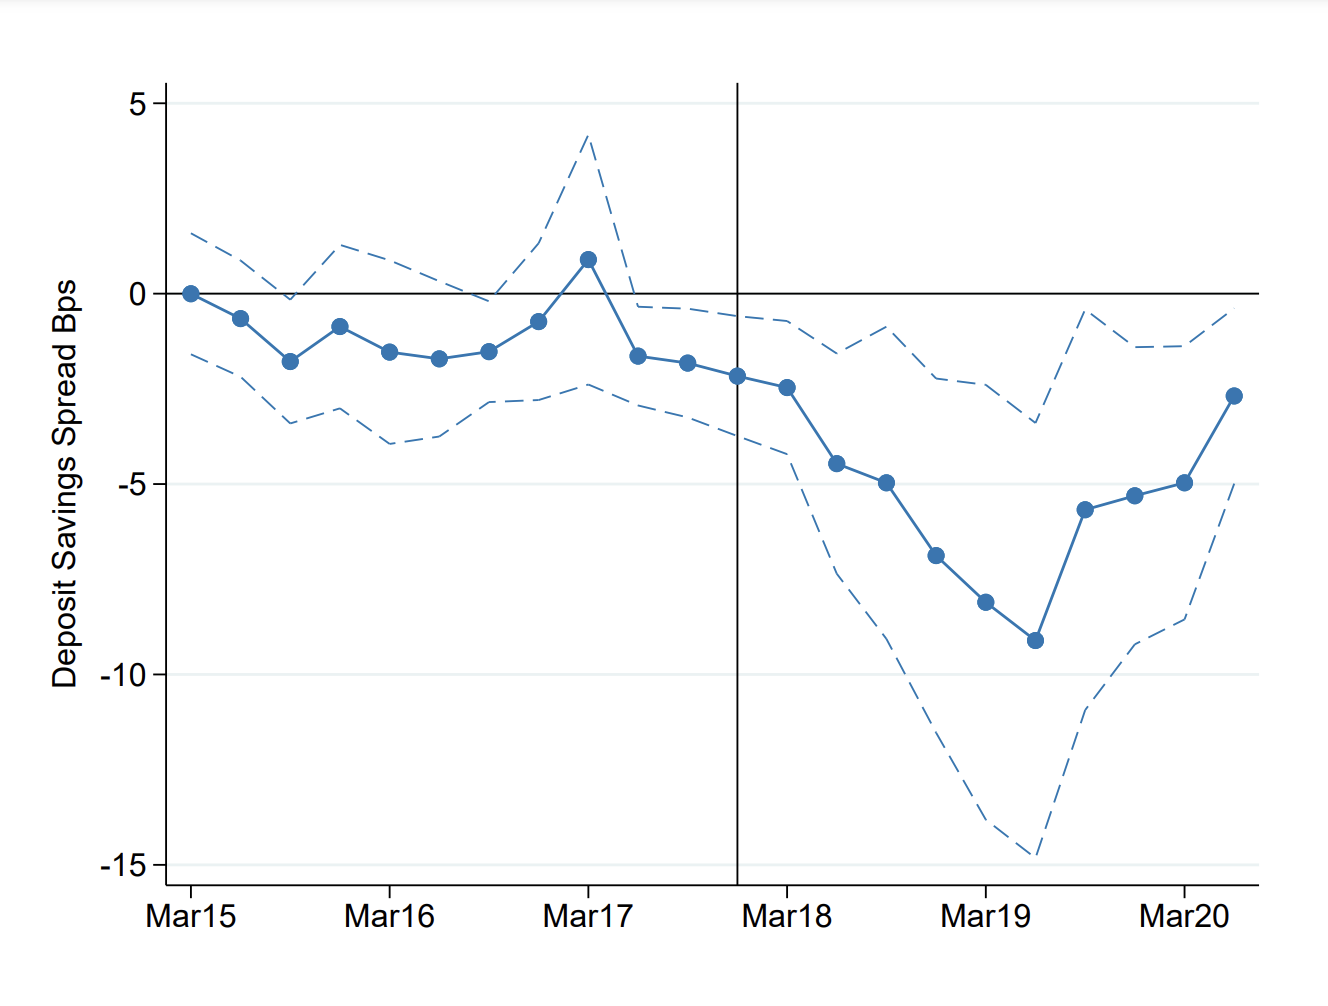
\includegraphics[width=.55\textwidth]{./imgs/figure7.png}
% \caption{Supply of Central Banks Reserves and Bank Asset Illiquidity}
\end{figure}

\end{frame}


\begin{frame}{Multimarket Contact and Retail Industries}

  \begin{wideitemize}
  \item Use data from Dun and Bradstreet (D\&B) and data on public firms from CRSP and Compustat.
  \item Constructs the sales portfolio using: 
  $$\hat{q}^i_c = \frac{\text{establishments}^i_c}{\sum_{j \in ind(i)} \text{establishments}^j_c}\text{population}_c$$
  where $\text{establishments}^i_c$ is the number of establishments of firm $i$ in county $c$ and $ind(i)$ is the industry of firm $i$.
\end{wideitemize}


\end{frame}


\begin{frame}{Multimarket Contact and Retail Industries}

  \begin{figure}[t*]
    \centering
    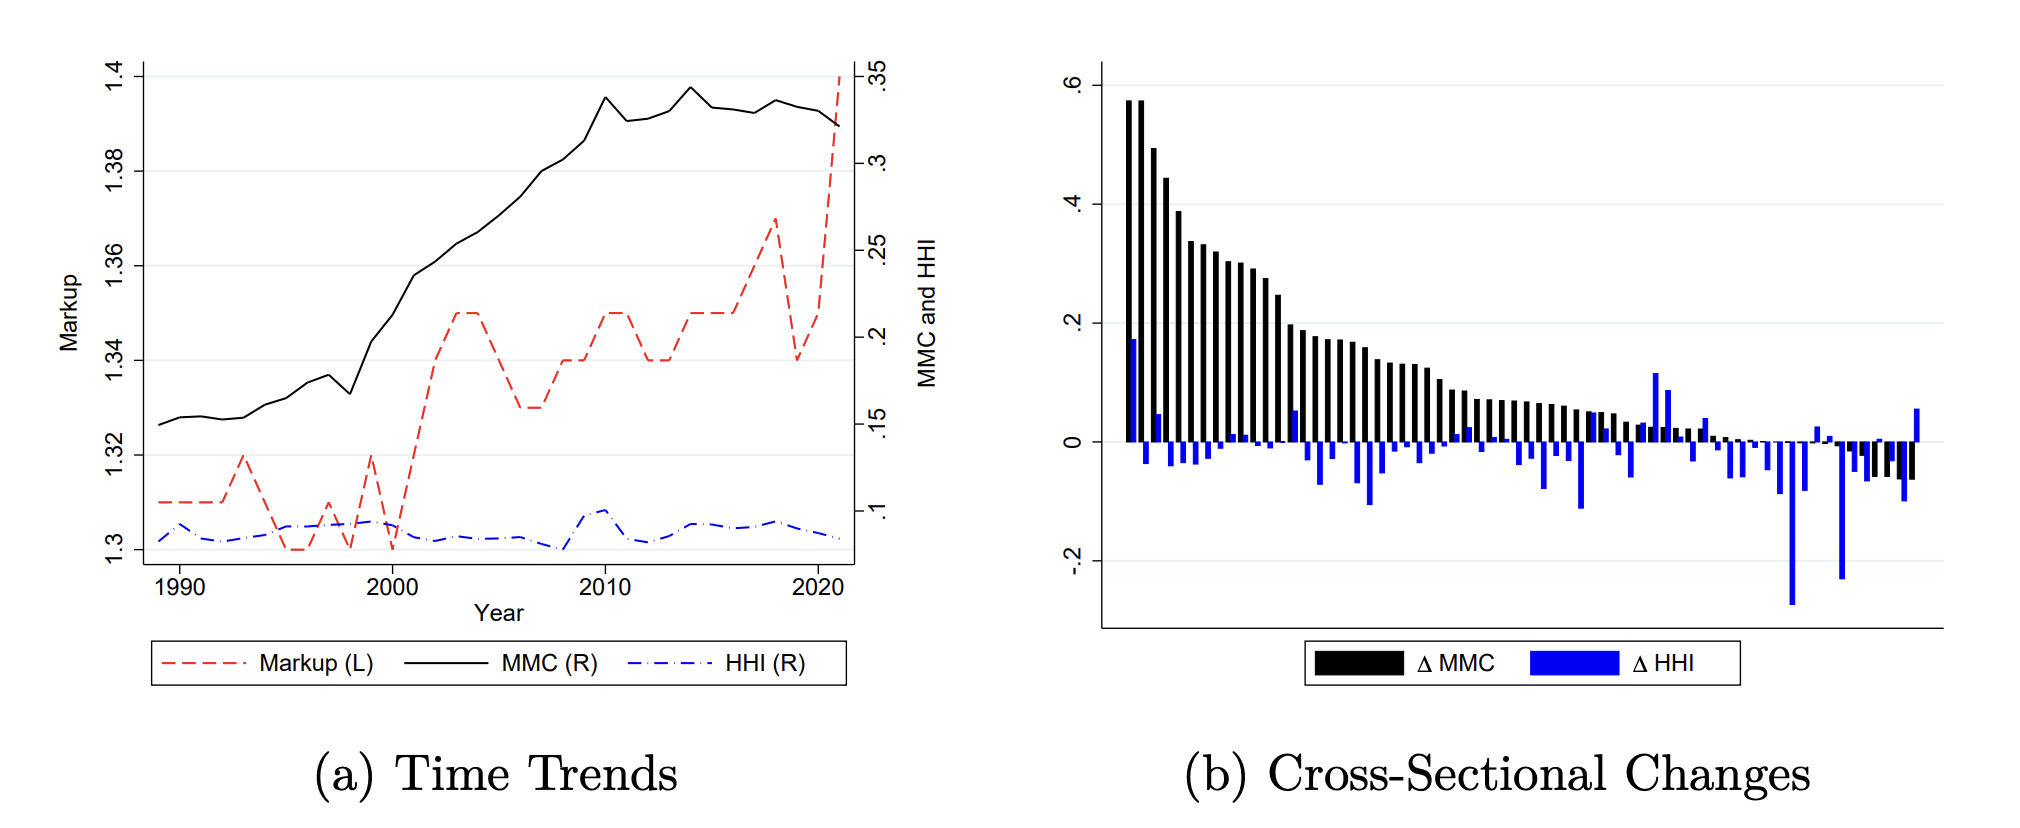
\includegraphics[width=.9\textwidth]{./imgs/figure4.png}
  % \caption{Supply of Central Banks Reserves and Bank Asset Illiquidity}
  \end{figure}
  
% TODO:  Figure 4
\end{frame}

      \begin{frame}[noframenumbering]
        \textcolor{blue}{\huge{\centerline{Conclusions}}}
    \end{frame}
    

      \begin{frame}{Conclusions}
        \vspace{0.5cm}
        \begin{wideitemize}
        \item Reconcile puzzle of U.S. deposit markets becoming less concentrated and less competitive. 
    \begin{wideitemize}
      \vspace{0.2cm}
        \item Banks' threat of competitive behavior in other markets to discipline behavior in markets with more competitors. 
        \item Overlaps reduce passthrough rate and increase markups. 
        \item Banks are twice as likely to merge into markets with high multimarket contact. 
 \end{wideitemize}

 \item Framework to studying how multimarket contact decreases competition.

        \item Antitrust regulators may need to consider multimarket contact when evaluating mergers.
      \end{wideitemize}
          
\end{frame}

\begin{frame}[noframenumbering]
\textcolor{blue}{\huge{\centerline{Thank you!}}}
\end{frame}

%\section*{References}
%\begin{frame}{References}
%    \bibliographystyle{plainnat}
%    \bibliography{references.bib}
%\end{frame}


% \end{frame}

\end{document}